\documentclass[headrule,landscape]{foils}

\usepackage{graphics}
\usepackage{color}
\usepackage{amsmath}
\usepackage{easyeqn}
\usepackage{epsfig}
\usepackage{amssymb}
\usepackage{rotating}
%\usepackage{pictex}

\newcommand{\noprint}[1]{}

%\setlength{\textwidth}{9.5in}
\setlength{\textheight}{7.2in}
\setlength{\topmargin}{-.5in}
%\setlength{\oddsidemargin}{.5in}

% shortcuts for colors
\definecolor{magenta4}{rgb}{.543,0,.543}
\definecolor{magenta3}{rgb}{.7,0,.7}
\definecolor{chartreuse4}{rgb}{.271,.545,0}
\definecolor{sienna}{rgb}{.627,.321,.176}
\definecolor{coral3}{rgb}{.803,.357,.271}
\definecolor{purple2}{rgb}{.569,.173,.933}
\definecolor{DarkGoldenrod3}{rgb}{.804,.584,.047}
\definecolor{DarkCyan}{cmyk}{.8, .2, 0, 0}
\def\blu#1{\textcolor{blue}{#1}}
\def\red#1{\textcolor{red}{#1}}
\def\mgn#1{\textcolor{magenta3}{#1}}
\def\grn#1{\textcolor{green}{#1}}
\def\cyn#1{\textcolor{cyan}{#1}}
\def\blk#1{\textcolor{black}{#1}}
\def\brn#1{\textcolor{sienna}{#1}}
\def\crl#1{\textcolor{coral3}{#1}}
\def\prp#1{\textcolor{purple2}{#1}}
\def\gld#1{\textcolor{DarkGoldenrod3}{#1}}

\newcommand{\foil}[1]{\foilhead[-.6in]{\blu{#1}}}
\newcommand{\rotatefoil}[1]{\rotatefoilhead[-.6in]{\blu{#1}}}
\newcommand{\overlay}[1]{\foilhead[-.6in]{\blu{\addtocounter{page}{-1}#1}}}
\newcommand{\bi}{\begin{itemize}}
\newcommand{\ei}{\end{itemize}}
\newcommand{\bb}{\item}
\newcommand{\bcyn}[1]{\item \cyn{#1}}
\newcommand{\bred}[1]{\item \red{#1}}
\newcommand{\emred}[1]{{\em \red{#1}}}
\newcommand{\emcyn}[1]{{\em \cyn{#1}}}
\newcommand{\m}[1]{\blu{$#1$}}
\newcommand{\one}{{\bf 1}}
\renewcommand{\Re}{{\mathbb R}}
\newcommand{\beq}[1]{\blu{\begin{equation*}#1\end{equation*}}}
\newtheorem{definition}{Definition}
\newtheorem{theorem}{Theorem}
\newtheorem{proposition}{Proposition}
\newtheorem{corollary}{Corollary}

%%%%%%%%%%%%%%%%%%%%%%%%%%%%%%%%%%%%%%%%%%%%%%%%%%%%%%%%%%%%%%%%%%%%%%%%%%%%%%%
\catcode`@=11 % enable private control sequences
%%%%%%%%%%%%%
\renewenvironment{itemize}[1][0pt]{%
  \ifnum \@itemdepth >\thr@@\@toodeep\else
    \advance\@itemdepth\@ne
    \edef\@itemitem{labelitem\romannumeral\the\@itemdepth}%
    \expandafter
    \list
      \csname\@itemitem\endcsname
      {\def\makelabel##1{\hss\llap{##1}}}\itemsep=#1%
  \fi
}{\endlist}
\let\enditemize=\endlist % for efficiency
%%%%%%%%%%%%%
\renewenvironment{enumerate}[1][0pt]{%
  \ifnum \@enumdepth >\thr@@\@toodeep\else
    \advance\@enumdepth\@ne
    \edef\@enumctr{enum\romannumeral\the\@enumdepth}%
      \expandafter
      \list
        \csname label\@enumctr\endcsname
        {\usecounter\@enumctr\def\makelabel##1{\hss\llap{##1}}\itemsep=#1%
  \fi}
}{\endlist}
\let\endenumerate =\endlist
%%%%%%%%%%%%%
\renewenvironment{description}[1][0pt]{%
  \list{}{\labelwidth\z@ \itemindent-\leftmargin
  \let\makelabel\descriptionlabel \itemsep=#1}
}{\endlist}
%%%%%%%%%%%%%
\catcode`\@=12 % disable private control sequences
%%%%%%%%%%%%%%%%%%%%%%%%%%%%%%%%%%%%%%%%%%%%%%%%%%%%%%%%%%%%%%%%%%%%%%%%%%%%%%%

\setlength{\parindent}{0pt}

%%%%%%%%%%%%%%%%%%%%%%%%%%%%%%%%%%%%%%%%%%%%%%%%%%%%%%%%%%%%%%%%%%%%%%%%%%%%%%%

\title{\blu{Parallel Solution of Vehicle Routing Problems} \\ \ \\}
%
\author{\cyn{Ted Ralphs} and \cyn{Ali Pilatin}\\ \ \\
\red{Industrial and Systems Engineering} \\ \red{Lehigh University} \\

\psfig{figure=/home/tkr/vrp_pics/F-n135-k7.ps,height=4.0in,angle=270}}
% title
% having the date is optional (as in standard LaTeX)
\date{\small \color{red} INFORMS Annual Meeting, November 16, 2005}
%
%\yourlogo{\Cyan{\ibmfont IBM}}     % This is the default
%\rightfooter{\quad{\sf\thepage}}   % This is the default
%\rightfooter{August 28, 2001}
\LogoOff  % We decided to turn the logo off 
\leftheader{INFORMS '05} 
\rightheader{\quad\textsf{\thepage}}
%\Restriction{ }

%%%%%%%%%%%%%%%%%%%%%%%%%%%%%%%%%%%%%%%%%%%%%%%%%%%%%%%%%%%%%%%%%%%%%%%%%%%%%%%

\begin{document}

%%%%%%%%%%%%%%%%%%%%%%%%%%%%%%%%%%%%%%%%%%%%%%%%%%%%%%%%%%%%%%%%%%%%%%%%%%%%%%%
%make the title page
\maketitle         % this makes the title page as usual

%%%%%%%%%%%%%%%%%%%%%%%%%%%%%%%%%%%%%%%%%%%%%%%%%%%%%%%%%%%%%%%%%%%%%%%%%%%%%%%

\foil{Outline of Talk}
%\large
\begin{tabular}{p{4in}p{4.5in}}
\bi
\bb Introduction
\bb A Tale of Two Methodologies
\bb Performance Measures
\bb Algorithm Design
\bb Computational Results?
\bb Future Directions
\ei
&
\begin{center}
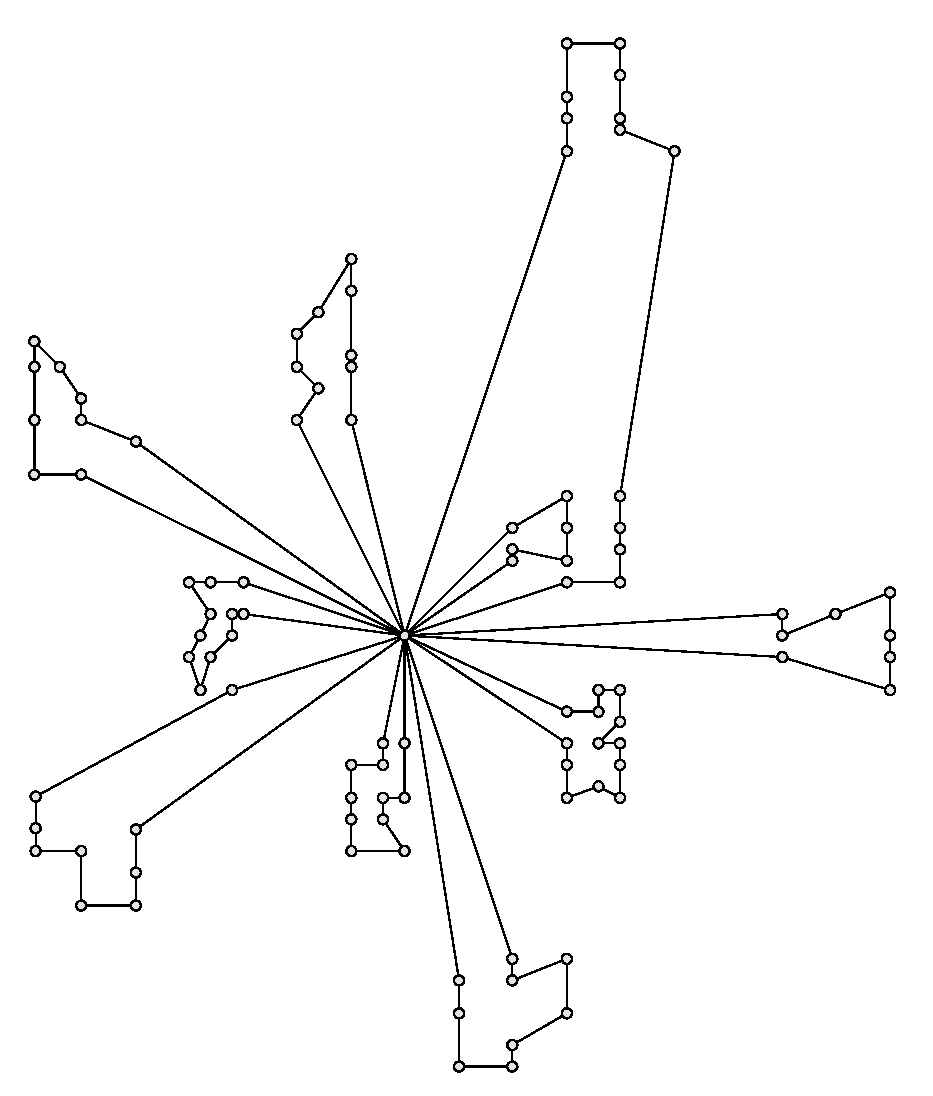
\psfig{figure=M-n101-k10-2.ps,height=5.0in}
\end{center}
\end{tabular}

%-----------------------------------------------------------------

\foil{The Project}

\bi
\bb \cyn{Goal}: To develop optimization software for use in a
commercial application for \red{automated vehicle location and routing}.
\bb \cyn{The Holy Grail}
\bi
\bb Good solutions in ``\red{real time}.''
\bb The ability to deal with real-time data ``\red{on the fly}.''
\ei
\bb \cyn{Toolbox}
\bi
\bb Heuristic methods
\bi
\bb Metaheuristics
\bb Primal heuristics
\ei
\bb ``Exact'' methods
\bi
\bb Warm starting
\bb Sensitivity analysis
\bb Decomposition
\ei
\bb Parallel/grid/on-demand computing
\ei
\bb \cyn{Challenge}: Create a \red{hybrid} technology that will use these
tools in a synergistic manner.
\ei

%-----------------------------------------------------------------

\foil{The Setting}

\bi
\bb \cyn{Target users} are small- and medium-sized delivery companies.
\bb We are interested in the usual variants of the \red{Vehicle Routing
  Problem}.
\bb \cyn{Customer static input data}
\bi
\bb Location
\bb Demand
\bb Time window
\bb Driver/vehicle restrictions
\ei
\bb \cyn{Fleet static input data}
\bi
\bb Number of trucks
\bb Truck capacities
\bb Route length restrictions
\bb Driver/vehicle descriptions
\ei
\bb Additional \red{real-time data} is available.
\bb The objective is to \red{minimize total driving distance/time}, subject to
appropriate constraints.
\ei

%-----------------------------------------------------------------

\foil{A Tale of Two Methodologies}

\bi
\bb ``It was the best of solutions, it was the worst of solutions...''
\bb \cyn{Heuristic methods} produce \emred{primal} information
\bi
\bb Primal solutions
\bb Upper bounds 
\bb Core variables
\ei
\bb \cyn{Exact methods} produce \emred{dual} information.
\bi
\bb Dual solutions
\bb Lower bounds
\bb Reduced costs
\ei
\bb The goal is to leverage this information in order to improve
overall performance.
\bb What do we mean by ``performance?''
\ei

%-----------------------------------------------------------------

\foil{Performance Measures}

\bi
\bb \cyn{What is the goal anyway}?
\bi
\bb Solve a given problem instance as quickly as possible.  
\bb Find the best possible solution in a fixed amount of time.
\bb Achieve the smallest possible gap in a fixed amount of time.
\bb Some combination...
\ei
\bb \cyn{Things to keep in mind}.
\bi
\bb The goal should be determined by the user.
\bb The method should be tailored to the goal.
\bb The goal may change as the solution procedure unfolds.
\ei
\bb Overall, we would like a \red{flexible methodological framework} that
adjusts to the user's requirements. 
\ei

%-----------------------------------------------------------------

\foil{A Bigger Hammer}

\bi
\bb The easiest way to achieve real-time performance is to use a
\red{bigger hammer} (parallel computng).
\bb Three phase \cyn{parallel} execution strategy
\bi
\bb \brn{Phase I}: Generate pool of initial solutions
\bb \brn{Phase II}: Improve pool with tabu search
\bb \brn{Phase III}: Close the gap (improve upper and lower bounds)
\ei
\bb Workers are allocated \red{dynamically} to perform one of three tasks
\bi
\bb Construct solutions from scratch
\bb Iteratively improve existing solutions
\bb Process subproblems arising from branch and cut
\ei
\bb Workers can be migrated from one task to another dynamically.
\bb As with any parallel algorithm, the key is \cyn{knowledge sharing}. 
\bb The goal is for branch and cut to work \red{symbiotically} 
with metaheuristic techniques. 
\ei

%-----------------------------------------------------------------

\foil{Architecture Summary}

\begin{center}
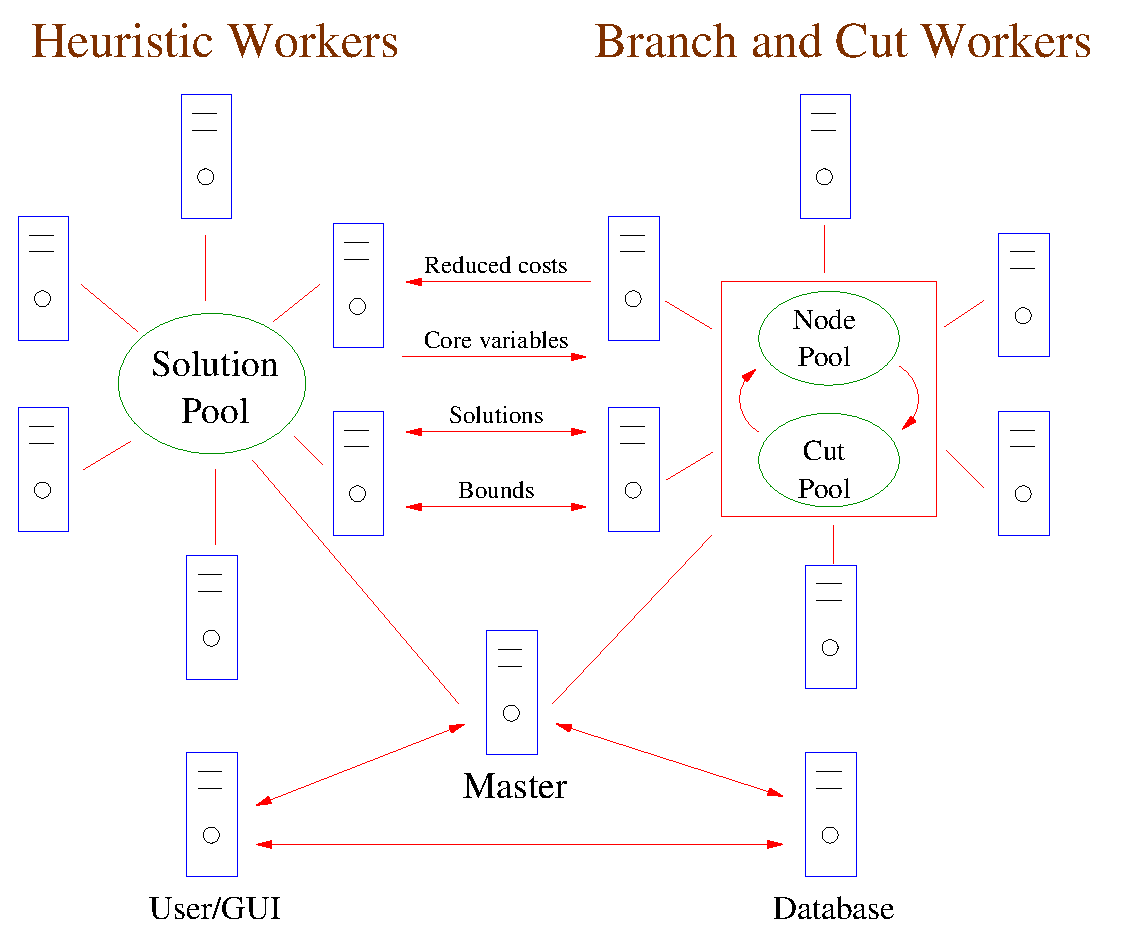
\psfig{figure=parallel.eps,height=6.0in}
\end{center}

%-----------------------------------------------------------------

\foil{Heuristics: Generating Initial Solutions}

\bi
\bb During \brn{Phase I}, all workers are dedicated to generating initial
solutions.  
\bb Initial generation is accomplished in several rounds.
\bi
\bb \underbar{\cyn{Clustering}}: Generate an initial pool of solutions using a
  variety of simple clustering heuristics.
\bb \underbar{\cyn{Routing}}: Improve initial routes for each of the clusters.   
\bb \underbar{\cyn{Exchange}}: Insert single customers on other routes
\bb \underbar{\cyn{Routing}}: Run route improvement routines again.
\bb \underbar{\cyn{Exchange}}: Exchange pairs of customers.
\bb \underbar{\cyn{Routing}}: Run route improvement routines once more.
\ei
\bb In the initial clustering, each worker executes one or
more heuristics and reports the results.
\bb The total number of heuristics to run is determined based on the size of
the problem and the number of available processors.
\bb The steps are optional and the pool of solutions can be reduced after each
step.
\ei 

%-----------------------------------------------------------------

\foil{Heuristics: Initial Solutions for the CVRP}

\bi
\bb \cyn{Clustering heuristics}
\bi
\bb Sweep
\bb Clarke and Wright
\bb Savings Insertion
\bb Near Cluster
\bb Route First, Cluster Second
\ei
\bb \cyn{Routing} is done using standard techniques for TSP tour construction.
\bb The first round of \cyn{exchange} checks to see whether single customers
can be inserted on other routes.
\bb The second round of \cyn{exchange} checks whether pairs of customers can
be swapped.
\ei

%-----------------------------------------------------------------

\noprint{

%Ali: leave this uncommented. I don't want to show it on the slides for the
%talk.

\foil{Heuristics: Initial Solutions for the CVRP}

\bi
\bb Clustering heuristics
  \bi
  \bb \bf{The sweep algorithm} This is a very simple heuristic for 
  clustering. 
  \bb Simply orders the nodes radially about the depot and 
  then adds to the current route in this order until capacity is 
  exceeded and then we start a new route. 
  \bb Depending on where we start in the cyclic ordering, we get 
  different solutions.
  \ei
\ei

\foil{Phase I/Clustering heuristics (cont'd)}
\bi
  \bb \bf{Clarke and Wright} This algorithm first places one customer 
  per route. 
  \bb At each iteration combines the routes that give the highest savings, 
  until capacitywise there is no feasible combination  anymore.
  \bb \bf{Savings Insertion} It starts by initiating the first route 
  by placing the initial starter (either the farthest node from the depot 
  of a random node) and the depot on the first route. 
  \bb at each iteration, it finds the customer with 
  the maximum savings among all customers not yet put on routes and 
  the the position in which to insert the customer in order to achieve 
  that savings. 
  \bb It then checks the feasibility of inserting that customer on the 
  most recent route being constructed and if it is infeasible, starts a 
  new route.
\ei

\foil{Phase I/Clustering heuristics (cont'd)}
\bi
  \bb \bf{Near Cluster} This algorithm builds all routes simultaneously. 
  \bb For each customer not already in the solution, it keeps track of 
  the route that it is closest to
  \bb At each step, the customer in closest proximity to its host
  route is added to that route and all distances are updated. 
  \bb If it is found to be infeasible to add the customer to the route, 
  then a new host is found and we start the process again.
\ei
\foil{Phase I/Clustering heuristics (cont'd)}
\bi
  \bb \bf{Route First, Cluster Second} These algorithms first construct a 
  heuristic TSP route and then partition it into feasible routes by 
  finding a shortest cycle of a graph with edge costs between nodes 
  being defined as the cost of a route from one endpoint of the edge 
  to the other.
  \bb They start by randomly choosing a node to be the first node on the 
  TSP tour.
  \bb There are three variations based on how the heuristic TSP tour is 
  constructed:
  \bi
    \bb \bf{(i)} at each iteration, farthest node from the nodes already
    inserted to the TSP tour is inserted
    \bb \bf{(ii)} at each iteration, nearest node to the nodes already
    inserted to the TSP tour is inserted
    \bb \bf{(iii)} until a parametric proportion of nodes are inserted
    in the TSP tour, insertion is as in \bf{(i)}, then it continues as in
    \bf{(ii)}.
  \ei
  \bb these heuristics are repeated for different starting nodes.
\ei
\bb \cyn{Routing} is done using standard techniques for TSP tour construction.
\bb The first round of \cyn{exchange} checks to see whether single customers
can be inserted on other routes.
\bb The second round of \cyn{exchange} checks whether pairs of customers can
be swapped.
\ei
}

%-----------------------------------------------------------------

\foil{Heuristics: Tabu Search}

\bi
\bb During \brn{Phase II}, all workers are dedicated to improving the most
promising solutions with tabu search.
\bb This is done in parallel, with one or more solutions assigned to each
available processor.
\bb \cyn{Dynamic tabu tenures} are used to handle diversification and
intensification.
\bb Dives into the infeasible region are allowed with the optional 
penalized tabu approach.
\bb At each iteration, the neighborhood is (currently) defined by one of four 
randomly chosen moves.
\bi 
\bb Moving a node within a route.
\bb Moving two nodes within a route.
\bb Moving a node to another route.
\bb Moving two nodes to other routes.
\ei
\ei

%-----------------------------------------------------------------

\foil{Exact Optimization: Branch and Cut}

\bi
\bb The branch and cut algorithm is implemented using SYMPHONY.
\bb \grn{SYMPHONY} is an open-source software package for solving and
analyzing mixed-integer linear programs (MILPs). 
\bb \grn{SYMPHONY} can be used in three distinct modes.
\bi
\bb \underbar{\cyn{Black box solver}}: Solve generic MILPs (command line or
shell).  
\bb \underbar{\cyn{Callable library}}: Call SYMPHONY from a C/C++ code.
\bb \underbar{\cyn{Framework}}: Develop a customized solver or
callable library with callbacks
\ei
\bb \grn{SYMPHONY} is part of the \red{Computational Infrastructure for
Operations Research} (COIN-OR) libraries (\brn{\texttt{www.coin-or.org}}).
\bb We have used \grn{SYMPHONY} to implement a solver customized for the
VRP.
\bb The solver is based on the standard two-index formulation and includes cut
generation, custom branching rules, etc. 
\bb If you want to know more about \grn{SYMPHONY}, check out session \red{WC}.
\ei

%-----------------------------------------------------------------

\foil{Exact Optimization: Parallelizing Branch and Cut}

\bi
\bb \grn{SYMPHONY} can be used in a variety of parallel execution modes.
\bb \grn{SYMPHONY} modules
\bi
\bb \cyn{Master}
\bb \cyn{Tree Manager} (TM)
\bb \cyn{Node Processor} (NP)
\bb \cyn{Cut Generator} (CG)
\bb \cyn{Cut Manager} (CM)
\ei
\bb These modules can be combined to form executables that work in concert to
perform branch and cut.
\bb We will use the following configuration.
\bi
\bb One \red{master} consisting of the \cyn{Master}, \cyn{TM}, and \cyn{CP}
modules.
\bb Multiple \red{workers} consisting of the \cyn{NP} and \cyn{CG} modules. 
\ei
\ei

%-----------------------------------------------------------------

\foil{Exact Optimization: Using the Solver}

\bi
\bb The exact solver can be used effectively for optimizing individual
routes.
\bi
\bb Small TSPs can be quickly solved to optimality.
\bb The routing step in initial solution generation is performed this way
\ei
\bb An exact TSP tour on all customer nodes can be used to initialize a
\cyn{route first, cluster second} method.
\bb In \brn{Phase III}, the exact solver can be used to:
\bi
\bb Provide performance guarantees (\cyn{lower bounds})
\bb Generate improved \cyn{primal solutions}
\bb Generate dual information to guide the heuristics
(\cyn{reduced costs}).
\ei
\ei

%-----------------------------------------------------------------

\foil{Exact Optimization: Core Variables}

\bi
\bb \grn{SYMPHONY} allows the designation of a problem \emred{core}.
\bi
\bb A set of ``important'' constraints. 
\bb A set of variables ``likely'' to appear in an optimal solution.
\ei
\bb Designating a core can improve the efficiency of branch and cut.
\bb Optimizing over the core can also be an effective heuristic technique.
\bb \grn{SYMPHONY} has a two-phase method in which the remaining variables are
``repriced'' in the root node. 
\bb This technique can be used to remove variables from the problem before
continuing the solution process.
\ei

%-----------------------------------------------------------------

\foil{Putting It All Together}

\bi
\bb In \brn{Phase III}, we can decide how many workers to allocate to each
pool.
\bb We can continue to construct new solutions, improve existing ones, or focus
on branch and cut.
\bb \red{Knowledge sharing} is the emphasis during this phase
\bb \cyn{Knowledge passed from heuristics to branch and cut}.
\bi
\bb The core is composed of the union of the best heuristically generated
tours. 
\bb The best solution found so far is used to initialize the upper bound.
\ei
\bb \cyn{Knowledge passed from branch and cut to heuristics}.
\bi
\bb Solutions found during the search process become candidates for tabu
search. 
\bb The indices of variables that have been fixed can also be passed to help
guide execution of the heuristics.
\bb Reduced costs and other dual information might be useful in guiding the
heuristics.
\ei
\ei

%-----------------------------------------------------------------

\foil{Extensions: Heuristics Based on Branch and Cut}

There are a number of ways in which ``incomplete'' branch and cut can be
used as a heuristic or a solution improvement procedure. 
\bi
\bb Switch to a search strategy emphasizing diving.
\bb Use a modified version of branch and cut to improve solutions
\bi
\bb RINS-based local search.
\bb Aggressive reduced-cost fixing.
\ei
\bb Since our goal is to find good solutions, default search parameters can be
modified to emphasize finding feasible solutions.
\ei
 
%-----------------------------------------------------------------

\foil{Extensions: Real-time Changes to Problem Data}

\bi
\bb We are currently exploring methodology for allowing dynamic changes to
problem data.
\bb By maintaining appropriate solution information, we can adjust the
solution procedure on the fly.
\bi
\bb Pools of feasible solutions (primal)
\bb Snapshots of the branch and cut tree (dual).
\ei
\bb For small changes, bound estimates can be obtained on the fly using
sensitivity analysis techniques.
\bb For larger changes, warm starting techniques can allow the solution
process to be restarted.
\bb Multicriteria and parametric optimization can be used to anticipate
future changes.
\ei

%-----------------------------------------------------------------

\foil{Computational Setup}

\bi
 \bb We tested the solver on a variety of instances from the libraries
maintained by \cyn{Ralphs} and \cyn{Vigo}.
 \bb The solver was deployed on a Beowulf cluster with 60 1.8 GHz 64-bit AMD
Opteron processors, each with 1G local memory. 
 \bb The communications protocol was PVM.
 \bb Testing was done with numbers of processors varied from 1 to 32.
 \bb Scaling strategy
 \bi
   \bb first a scaling multiplier is calculated that is directly proportional
    to the number of processors, and inversely proportional to square of the 
    number of vertices in the instance 
   \bb \brn{Phase I}: The number of clustering heuristics is scaled with the
 number of processors.
\bb \brn{Phase II}: Each processor received one solution to improve with tabu
search.
\bb \brn{Phase III}: Exact solver was run with a time limit equal to twice the
number of vertices.
\ei
\ei

%-----------------------------------------------------------------

\foil{Computational Results: Best Clustering Strategies}

\begin{center}
\begin{tabular}{||l|l||}
\hline
Heuristic & Average Percent over Best\\\hline\hline
TSP (FINI) & 0.558991\\\hline
TSP (FI) & 1.17818\\\hline
TSP (NI) & 2.21181\\\hline
Clarke and Wright & 3.01447\\\hline
Savings Insertion I & 13.8535\\\hline
Savings Insertion II & 13.6061\\\hline
\hline
\end{tabular}
\end{center}

%-----------------------------------------------------------------

\foil{Computational Results: Effect of Parallelism on Gap}
\begin{center}
\begin{tabular}{||l|l||}
\hline
Processors & Avg Final Gap without Using Core Variables \\\hline\hline
1 & 1.87\\\hline
4 & 1.60 \\\hline
8 & 1.37 \\\hline
16 & 1.23 \\\hline
32 & 1.20 \\\hline
\hline
\end{tabular}
\end{center}

%-----------------------------------------------------------------

\noprint{
\foil{Computational Results: Scalability of SYMPHONY (No Bounds)}

{\tiny
%\begin{table}
$$
\begin{array}{|l|r|r|r|r|r|r|r|r|r|r|}
\hline
{\rm Instance} & {\rm Tree}
  & {\rm Ramp}
  & {\rm Ramp}
  & {\rm Node}
  & {\rm Idle}
  & {\rm Idle}
  & {\rm Idle}
  & {\rm CPU} & {\rm Wallclock} 
  & {\rm Eff} \\
& {\rm Size}
  & {\rm Up}
  & {\rm Down}
  & {\rm Pack}
  & {\rm Node}
  & {\rm Index}
  & {\rm Diving}
  & {\rm sec} & 
  &  \\
\hline
{\rm hk48-n48-k4} & 110 & 0.00 & 0.00 & 0.00 & 0.02 & 0.01 & 0.01 & 17.88 & 18.46 & \\
{\rm att-n48-k4} & 292 & 0.00 & 0.00 & 0.00 & 0.05 & 0.03 & 0.04 & 29.37 & 30.34 & \\
{\rm E-n51-k5} & 38 & 0.00 & 0.00 & 0.00 & 0.01 & 0.01 & 0.00 & 13.29 & 13.88 & \\
{\rm A-n39-k5} & 1139 & 0.00 & 0.00 & 0.03 & 0.13 & 0.14 & 0.12 & 218.66 & 226.46 & \\
{\rm A-n39-k6} & 273 & 0.00 & 0.00 & 0.00 & 0.04 & 0.03 & 0.03 & 26.88 & 27.53 & \\
{\rm A-n45-k6} & 807 & 0.00 & 0.00 & 0.02 & 0.14 & 0.13 & 0.10 & 247.97 & 257.05 & \\
{\rm A-n46-k7} & 83 & 0.00 & 0.00 & 0.00 & 0.01 & 0.02 & 0.01 & 45.01 & 47.51 & \\
{\rm B-n34-k5} & 1101 & 0.00 & 0.00 & 0.02 & 0.10 & 0.10 & 0.11 & 41.66 & 43.15 & \\
{\rm B-n43-k6} & 197 & 0.00 & 0.00 & 0.01 & 0.04 & 0.03 & 0.02 & 27.52 & 28.54 & \\
{\rm B-n45-k5} & 126 & 0.00 & 0.00 & 0.00 & 0.02 & 0.02 & 0.02 & 17.92 & 18.48 & \\
{\rm B-n51-k7} & 327 & 0.00 & 0.00 & 0.01 & 0.09 & 0.05 & 0.05 & 47.01 & 48.75 & \\
{\rm B-n64-k9} & 137 & 0.00 & 0.00 & 0.01 & 0.03 & 0.02 & 0.02 & 39.41 & 40.83 & \\
{\rm A-n53-k7} & 1682 & 0.00 & 0.00 & 0.08 & 0.63 & 0.21 & 0.17 & 698.52 & 735.62 & \\
{\rm A-n44-k6} & 5233 & 0.00 & 0.00 & 0.20 & 1.13 & 0.79 & 0.73 & 1471.47 & 1523.40 & \\
{\rm B-n45-k6} & 5413 & 0.00 & 0.00 & 0.18 & 0.95 & 0.82 & 0.81 & 1115.43 & 1157.26 & \\
\hline
{\rm 1\;NP} & 16958 & 0.00 & 0.00 & 0.56 & 3.40 & 2.40 & 2.26 & 4058.00 &
4217.26 & 1.00 \\
\hline
%{\rm Per\;Node} & & 0.0000 & 0.0000 & 0.0000 & 0.0002 & 0.0001 & 0.0001 & 0.2393 & 0.2487 & \\
%\hline
{\rm 2\;NP's} & 16918 & 16.61 & 0.00 & 0.55 & 3.73 & 2.54 & 2.36 & 4051.79 &
2115.68 & 1.00  \\
\hline
%{\rm Per\;Node} & & 0.0010 & 0.0000 & 0.0000 & 0.0002 & 0.0001 & 0.0001 & 0.2395 & 0.2501 & \\
%\hline
{\rm 4\;NP's} & 16933 & 68.54 & 0.00 & 0.54 & 4.02 & 2.41 & 2.25 & 4030.29 &
1066.63 & 0.99 \\
\hline
%{\rm Per\;Node} & & 0.0040 & 0.0000 & 0.0000 & 0.0002 & 0.0001 & 0.0001 & 0.2380 & 0.2520 & \\
%\hline
{\rm 8\;NP's} & 16891 & 199.20 & 1.02 & 0.54 & 4.27 & 2.56 & 2.40 & 4031.21 &
551.15 & 0.96 \\
\hline
%{\rm Per\;Node} & & 0.0118 & 0.0001 & 0.0000 & 0.0003 & 0.0002 & 0.0001 & 0.2387 & 0.2610 & \\
%\hline
{\rm 16\;NP's} & 18715 & 513.93 & 29.95 & 0.58 & 7.29 & 2.97 & 2.84 & 4520.36
& 330.86 & 0.80 \\
\hline
%{\rm Per\;Node} & & 0.0275 & 0.0016 & 0.0000 & 0.0004 & 0.0002 & 0.0002 & 0.2415 & 0.2829 & \\
%\hline
{\rm 32\;NP's} & 16160 & 1249.31 & 75.52 & 1.42 & 60.44 & 81.97 & 78.37 &
3781.30 & 176.54 & 0.75 \\
\hline
%{\rm Per\;Node} & & 0.0773 & 0.0047 & 0.0001 & 0.0037 & 0.0051 & 0.0048 & 0.2340 & 0.3496 & \\
%\hline
\end{array}
$$
%\caption{Solving VRP instances with SYMPHONY: Default settings and no a priori
%  upper bound (summary) \label{tab:default-vrp}}
%\end{table}
}
}

%-----------------------------------------------------------------

\foil{Computational Results: Scalability of SYMPHONY VRP Solver}

{\tiny
%\begin{table}
$$
\begin{array}{|l|r|r|r|r|r|r|r|r|r|r|}
\hline
& {\rm Tree}
  & {\rm Ramp}
  & {\rm Ramp}
  & {\rm Node}
  & {\rm Idle}
  & {\rm Idle}
  & {\rm Idle}
  & {\rm CPU} & {\rm Wallclock} 
  & {\rm Eff} \\
{\rm Instance} & {\rm Size}
  & {\rm Up}
  & {\rm Down}
  & {\rm Pack}
  & {\rm Node}
  & {\rm Index}
  & {\rm Diving}
  & {\rm sec} & 
  &  \\
\hline
{\rm hk48-n48-k4} & 110 & 0.00 & 0.00 & 0.00 & 0.03 & 0.01 & 0.01 & 16.77 & 17.35 & \\
{\rm att-n48-k4} & 384 & 0.00 & 0.00 & 0.01 & 0.05 & 0.04 & 0.05 & 36.61 & 37.77 & \\
{\rm E-n51-k5} & 41 & 0.00 & 0.00 & 0.00 & 0.01 & 0.01 & 0.01 & 14.86 & 15.49 & \\
{\rm A-n39-k5} & 1307 & 0.00 & 0.00 & 0.04 & 0.23 & 0.18 & 0.15 & 242.33 & 251.04 & \\
{\rm A-n39-k6} & 328 & 0.00 & 0.00 & 0.01 & 0.07 & 0.04 & 0.03 & 31.95 & 32.66 & \\
{\rm A-n45-k6} & 631 & 0.00 & 0.00 & 0.02 & 0.13 & 0.08 & 0.07 & 175.12 & 181.64 & \\
{\rm A-n46-k7} & 43 & 0.00 & 0.00 & 0.00 & 0.01 & 0.01 & 0.00 & 15.03 & 15.71 & \\
{\rm B-n34-k5} & 795 & 0.00 & 0.00 & 0.01 & 0.10 & 0.08 & 0.09 & 29.99 & 31.08 & \\
{\rm B-n43-k6} & 288 & 0.00 & 0.00 & 0.01 & 0.05 & 0.04 & 0.03 & 38.24 & 39.67 & \\
{\rm B-n45-k5} & 133 & 0.00 & 0.00 & 0.00 & 0.02 & 0.02 & 0.02 & 15.69 & 16.21 & \\
{\rm B-n51-k7} & 367 & 0.00 & 0.00 & 0.01 & 0.12 & 0.05 & 0.05 & 53.50 & 55.37 & \\
{\rm B-n64-k9} & 152 & 0.00 & 0.00 & 0.00 & 0.03 & 0.02 & 0.02 & 44.00 & 46.12 & \\
{\rm A-n53-k7} & 3056 & 0.00 & 0.00 & 0.17 & 1.16 & 0.39 & 0.33 & 1295.06 & 1362.33 & \\
{\rm A-n37-k6} & 5873 & 0.00 & 0.00 & 0.21 & 1.36 & 0.73 & 0.67 & 832.46 & 857.40 & \\
{\rm A-n44-k6} & 5963 & 0.00 & 0.00 & 0.31 & 1.95 & 0.80 & 0.67 & 1677.44 & 1741.78 & \\
{\rm B-n45-k6} & 2039 & 0.00 & 0.00 & 0.07 & 0.46 & 0.28 & 0.23 & 379.23 & 394.49 & \\
{\rm B-n57-k7} & 3205 & 0.00 & 0.00 & 0.17 & 1.11 & 0.42 & 0.41 & 976.52 & 1036.09 & \\
\hline
{\rm 1\;NP} & 24715 & 0.00 & 0.00 & 1.03 & 6.89 & 3.20 & 2.86 & 5874.80 &
6132.22 & 1.00 \\
\hline
%{\rm Per\;Node} & & 0.0000 & 0.0000 & 0.0000 & 0.0003 & 0.0001 & 0.0001 & 0.2377 & 0.2481 & \\
%\hline
{\rm 2\;NP's} & 24680 & 19.48 & 0.00 & 1.01 & 6.65 & 3.18 & 2.91 & 5832.25 &
3054.99 & 1.01 \\
\hline
%{\rm Per\;Node} & & 0.0008 & 0.0000 & 0.0000 & 0.0003 & 0.0001 & 0.0001 & 0.2363 & 0.2476 & \\
%\hline
{\rm 4\;NP's} & 23930 & 74.77 & 0.00 & 0.96 & 7.03 & 3.05 & 2.73 & 5620.94 &
1488.74 & 1.03 \\
\hline
%{\rm Per\;Node} & & 0.0031 & 0.0000 & 0.0000 & 0.0003 & 0.0001 & 0.0001 & 0.2349 & 0.2488 & \\
%\hline
{\rm 8\;NP's} & 24366 & 221.67 & 3.56 & 0.97 & 8.41 & 3.36 & 3.00 & 5701.00 &
774.99 & 0.99 \\
\hline
%{\rm Per\;Node} & & 0.0091 & 0.0001 & 0.0000 & 0.0003 & 0.0001 & 0.0001 & 0.2340 & 0.2544 & \\
%\hline
{\rm 16\;NP's} & 25668 & 572.93 & 11.83 & 0.98 & 11.52 & 3.75 & 3.51 & 6090.37
& 437.66 & 0.87 \\
\hline
%{\rm Per\;Node} & & 0.0223 & 0.0005 & 0.0000 & 0.0004 & 0.0001 & 0.0001 & 0.2373 & 0.2728 & \\
%\hline
{\rm 32\;NP's} & 25516 & 1416.55 & 60.98 & 3.02 & 113.66 & 121.30 & 110.45 &
5998.93 & 257.71 & 0.74 \\
\hline
%{\rm Per\;Node} & & 0.0555 & 0.0024 & 0.0001 & 0.0045 & 0.0048 & 0.0043 & 0.2351 & 0.3232 & \\
%\hline
\end{array}
$$
%\caption{Solving VRP instances with SYMPHONY: Default settings and
%  heuristic upper bound (summary) \label{tab:ub-vrp-1}}
%\end{table}
}

%-----------------------------------------------------------------

\noprint{
\foil{Computational Results: Scalability of SYMPHONY}

\begin{sidewaystable}
$$
\begin{array}{|l|r|r|r|r|r|r|r|r|r|}
\hline
{\rm Instance} & {\rm Tree\ Size}
  & {\rm Ramp\ Up}
  & {\rm Ramp\ Down}
  & {\rm Node\ Pack}
  & {\rm Idle\ Node}
  & {\rm Idle\ Index}
  & {\rm Idle\ Diving}
  & {\rm CPU\ sec} & {\rm Wallclock} \\
\hline
{\rm hk48-n48-k4} & 178 & 59.11 & 2.78 & 0.01 & 0.46 & 1.20 & 0.91 & 26.11 & 3.06\\
{\rm att-n48-k4} & 349 & 34.03 & 0.04 & 0.01 & 0.75 & 1.51 & 1.29 & 32.45 & 2.53\\
{\rm E-n51-k5} & 37 & 74.11 & 0.00 & 0.00 & 0.05 & 0.05 & 0.06 & 13.82 & 3.24\\
{\rm A-n39-k5} & 1228 & 99.86 & 0.04 & 0.06 & 4.11 & 6.57 & 5.99 & 232.97 & 11.36\\
{\rm A-n39-k6} & 328 & 35.52 & 9.34 & 0.01 & 0.99 & 1.23 & 0.98 & 32.02 & 2.75\\
{\rm A-n45-k6} & 727 & 105.07 & 0.08 & 0.06 & 2.71 & 3.38 & 2.64 & 215.34 & 10.96\\
{\rm A-n46-k7} & 36 & 157.81 & 0.00 & 0.00 & 1.19 & 0.04 & 0.03 & 13.93 & 5.53\\
{\rm B-n34-k5} & 859 & 10.77 & 0.01 & 0.02 & 1.34 & 1.69 & 2.34 & 32.36 & 1.68\\
{\rm B-n43-k6} & 296 & 65.73 & 6.82 & 0.02 & 3.32 & 1.16 & 0.94 & 37.50 & 3.68\\
{\rm B-n45-k5} & 179 & 72.23 & 7.21 & 0.01 & 1.75 & 0.50 & 0.48 & 20.82 & 3.72\\
{\rm B-n51-k7} & 365 & 41.01 & 12.07 & 0.02 & 2.05 & 1.66 & 1.39 & 52.84 & 3.79\\
{\rm B-n64-k9} & 136 & 158.05 & 0.00 & 0.04 & 3.51 & 0.85 & 0.70 & 36.11 & 6.59\\
{\rm A-n53-k7} & 3012 & 178.18 & 0.53 & 0.45 & 14.87 & 12.61 & 11.52 & 1278.10 & 49.22\\
{\rm A-n37-k6} & 5999 & 54.78 & 12.96 & 0.51 & 23.60 & 27.99 & 24.62 & 849.45 & 32.03\\
{\rm A-n44-k6} & 5916 & 115.84 & 1.03 & 0.79 & 28.99 & 30.29 & 27.20 & 1667.73 & 60.78\\
{\rm B-n45-k6} & 1991 & 74.93 & 0.32 & 0.26 & 8.53 & 11.16 & 9.86 & 372.13 & 16.08\\
{\rm B-n57-k7} & 3877 & 79.51 & 7.76 & 0.73 & 15.44 & 19.40 & 19.49 & 1085.24 & 40.73\\
\hline
{\rm 32\;NP's} & 25516 & 1416.55 & 60.98 & 3.02 & 113.66 & 121.30 & 110.45 & 5998.93 & 257.71\\
\hline
%{\rm Per\;Node} & & 0.0555 & 0.0024 & 0.0001 & 0.0045 & 0.0048 & 0.0043 & 0.2351 & 0.3232\\
%\hline
\end{array}
$$
\caption{Solving VRP instances with SYMPHONY: Default settings and
  heuristic upper bound (32 NPs) \label{tab:ub-vrp-2}}
\end{sidewaystable}
}

%-----------------------------------------------------------------

\noprint{
\foil{Computational Results: Effect of Tabu Search}
\bi
\bb Avg. Tabu Search Improvement Over the Initial Heuristics
\ei
\begin{center}
\begin{tabular}{||l|l||}
\hline
Processors & Tabu Search Improvement\\\hline\hline
1 & 0\\\hline
4 & 0\\\hline
8 & 0\\\hline
16 & 0\\\hline
32 & 0\\\hline
%1 & 0\\\hline
%4 & 0.0851465\\\hline
%8 & 0.108079\\\hline
%16 & 0.230457\\\hline
%32 & 0.247085\\\hline
\hline
\end{tabular}
\end{center}

%-----------------------------------------------------------------

%\foil{Computational Reslts: Effect of Upper Bound}
%\bi
%\bb Average Effect of Heuristic U.B. in Improving the Optimality Gap
%\ei
%\begin{center}
%\begin{tabular}{||l|l||}
%\hline
%Processors & Gap Improvement\\\hline\hline
%1 & 99.9994\\\hline
%4 & 99.9992\\\hline
%8 & 99.999\\\hline
%16 & 99.9992\\\hline
%32 & 99.999\\\hline
\hline
\end{tabular}
\end{center}

%-----------------------------------------------------------------

\foil{Computational Results: Effect of Core Variables on Gap}
\bi
\bb Avg Improvement of optimality gap by using core variables in SYMPHONY
\ei
\begin{center}
\begin{tabular}{||l|l||}
\hline
Processors & Gap Improvement by Core Variables \\\hline\hline
1 & 28.5714\\\hline
4 & 8.33333\\\hline
8 & -2.43902\\\hline
16 & -8.10811\\\hline
32 & -8.33333\\\hline
\hline
\end{tabular}
\end{center}

%-----------------------------------------------------------------
\foil{Computational Results: Effect of Core Variables on UB}
\bi
\bb Avg Improvement of UB by using core variables in SYMPHONY
\ei
\begin{center}
\begin{tabular}{||l|l||}
\hline
Processors & UB Improvement by Core Variables \\\hline\hline
1 & -0.0328359\\\hline
4 & -12.4457\\\hline
8 & -4.70617\\\hline
16 & -12.6269\\\hline
32 & -7.93382\\\hline
\hline
\end{tabular}
\end{center}

%-----------------------------------------------------------------
\foil{Computational Results: Effect of Processors on Gap (E on)}
\begin{center}
\begin{tabular}{||l|l||}
\hline
Processors & Avg Final Gap Using Core Variables\\\hline\hline
1 & 1.33333\\\hline
4 & 1.46667\\\hline
8 & 1.4\\\hline
16 & 1.33333\\\hline
32 & 1.3\\\hline
\hline
\end{tabular}
\end{center}

%-----------------------------------------------------------------
\foil{Computational Results: Exact Solution UB improvement(E on)}
\begin{center}
\begin{tabular}{||l|l||}
\hline
Processors & Exact Solution UB improvement\\\hline\hline
1 & 0.515871\\\hline
4 & 0.664202\\\hline
8 & 0.51248\\\hline
16 & 0.537896\\\hline
32 & 0.541286\\\hline
\hline
\end{tabular}
\end{center}

%-----------------------------------------------------------------
\foil{Computational Results: Exact Solution UB improvement(E off)}
\begin{center}
\begin{tabular}{||l|l||}
\hline
Processors & Exact Solution UB improvement\\\hline\hline
1 & 0.674927\\\hline
4 & 0.917775\\\hline
8 & 0.884045\\\hline
16 & 0.909502\\\hline
32 & 0.91426\\\hline
\hline
\end{tabular}
\end{center}
}

%-----------------------------------------------------------------

\foil{Computational Results: Early Lessons}

\bi
\bb The exact optimization phase does seem to improve solutions in many cases,
but the computational cost.is high.
\bb We need to further develop heuristic variants of branch and cut.
\bb Using exact TSP optimization seems to lead to significant
improvement in initial solutions.
\bb For relatively small instances, optimizing over the core variables does
not seem to help much.
\bb This may nto be the case for larger instances.
\bb There is much more work to be done.
\ei

%-----------------------------------------------------------------

\foil{Conclusions and Future Work}

\bi
\bb This work is part of a much bigger ongoing effort to develop \red{real-time
solution procedures} for IP.
\bb Our goal is to make IP a \red{tactical} decision-making tool. 
\bb Our experience so far indicates that this will be a fruitful, but
challenging area of research.
\bb Parallel and grid computing technologies are a big enabler. 
\bb Heuristic solution techniques can be combined with exact solution
techniques in useful ways to improve overall performance. 
\ei

\end{document}

%-----------------------------------------------------------------

\foil{How Hard is the VRP?}
\bi
\bb {\color{blue} Test Set}
        \bi
        \bb {\color{green} TSPLIB/VRPLIB}
        \bb Augerat's repository
        \bb Available at {\tt \color{red} BranchAndCut.org/VRP}
        \ei
\bb Largest {\color{green} VRP} instance solved: {\color{blue} F-n135-k7}
\bb Largest {\color{green} TSP} instance solved: {\color{blue} d15112}
\bb Smallest {\color{green} VRP} instance unsolved (as of '01): 
{\color{blue} B-n50-k8}
\bb Time to solve {\color{blue} B-n50-k8} as an {\color{green} MTSP}: .1 sec
\bb {\color{red} Why the gap?}
\ei
%\begin{center}
%\psfig{figure=/home2/tkr/vrp_pics/A-n53-k7-2.ps,height=2.0in}
%\end{center}

%-----------------------------------------------------------------

\foil{Standard Approach}
\bi
\bb Standard approaches treat the \grn{VRP} in much the same way as the 
\grn{TSP}.
\bi
\bb Most known valid inequalities are generalizations from the \grn{TSP}.
\bb Branching rules are also generalizations from the \grn{TSP}.
\ei
\bb However, the TSP does not seem to be the right template.
\bb It is the packing, not the routing that makes the problem difficult.
\ei

%-----------------------------------------------------------------

\foil{}
\begin{center}
\psfig{figure=/home2/tkr/vrp_pics/B-n50-k8.ps,height=5.0in,angle=-90}
\end{center}

%-----------------------------------------------------------------

\foil{}
\begin{center}
\psfig{figure=/home2/tkr/vrp_pics/B-n50-k8.mtsp.ps,height=5.0in,angle=-90}
\end{center}

%-----------------------------------------------------------------

\foil{}
\begin{center}
\psfig{figure=/home2/tkr/vrp_pics/B-n50-k8-sol10.ps,height=5.0in,angle=-90}
\end{center}

%-----------------------------------------------------------------

\foil{}
\begin{center}
\psfig{figure=/home2/tkr/vrp_pics/E-n76-k7.mtsp2.ps,height=5.0in}
\end{center}

%-----------------------------------------------------------------

\foil{}
\begin{center}
\psfig{figure=/home2/tkr/vrp_pics/opt-E-n76-k7.ps,height=5.0in}
\end{center}

%-----------------------------------------------------------------

\foil{What Makes the VRP Difficult?}

\bi
\bb It is the intersection of two difficult problems.
\bi
\bb {\color{green} Traveling Salesman Problem} ({\color{blue} Routing})
\bb {\color{green} Bin Packing Problem} ({\color{blue} Packing})
\ei
\bb We don't have an effective, polynomially sized relaxation.
\bb Current approaches treat it as a {\color{red} routing} problem.
\bb We know very little about the {\color{red} packing} aspect.
\bb We need a different \grn{template}.
\bb \underbar{\color{red} Idea}: Consider flow-based formulations.
\ei
\begin{center}
\psfig{figure=/home2/tkr/Talks/pics/routing4.eps,height=1.8in}
\end{center}

%-----------------------------------------------------------------
\foil{Test Results}
\bi
\bb Performance comparison of Construction Heuristics
\ei
\begin{center}
\begin{tabular}{||l|l|l||}
\hline
Heuristic & Processors & Avg Worseness wrt the best\\\hline\hline
43 & 1 & 0.493871\\\hline
42 & 1 & 1.29684\\\hline
44 & 1 & 2.30184\\\hline
40 & 1 & 3.06797\\\hline
38 & 1 & 11.536\\\hline
37 & 1 & 12.9373\\\hline
40 & 4 & 1.92747\\\hline
42 & 4 & 2.00652\\\hline
43 & 4 & 2.9417\\\hline
44 & 4 & 3.05538\\\hline
37 & 4 & 11.8595\\\hline
38 & 4 & 14.5505\\\hline
42 & 8 & 2.12031\\\hline
40 & 8 & 2.39108\\\hline
43 & 8 & 3.26123\\\hline
44 & 8 & 4.60448\\\hline
37 & 8 & 11.8815\\\hline
38 & 8 & 14.6543\\\hline
42 & 16 & 1.97656\\\hline
40 & 16 & 2.39726\\\hline
43 & 16 & 3.29186\\\hline
44 & 16 & 4.85082\\\hline
37 & 16 & 13.0986\\\hline
38 & 16 & 24.0096\\\hline
42 & 32 & 1.98459\\\hline
40 & 32 & 2.40569\\\hline
43 & 32 & 3.29968\\\hline
44 & 32 & 4.85791\\\hline
37 & 32 & 18.9062\\\hline
38 & 32 & 41.1787\\\hline
\hline
\end{tabular}
\end{center}

\foil{Test Results (cont'd)}
\bi
\bb Avg. Tabu Search Improvement Over the Initial Heuristics
\ei
\begin{center}
\begin{tabular}{||l|l||}
\hline
Processors & Tabu Search Improvement\\\hline\hline
1 & 0\\\hline
4 & 0.0851465\\\hline
8 & 0.108079\\\hline
16 & 0.230457\\\hline
32 & 0.247085\\\hline
\hline
\end{tabular}
\end{center}

\foil{Test Results (cont'd)}
\bi
\bb Average Effect of Heuristic U.B. in Improving the Optimality Gap
\ei
\begin{center}
\begin{tabular}{||l|l||}
\hline
Processors & Gap Improvement\\\hline\hline
1 & 99.9994\\\hline
4 & 99.9992\\\hline
8 & 99.999\\\hline
16 & 99.9992\\\hline
32 & 99.999\\\hline
\hline
\end{tabular}
\end{center}

\foil{Test Results (cont'd)}
\bi
\bb Avg Improvement of optimality gap by using core variables in SYMPHONY
\ei
\begin{center}
\begin{tabular}{||l|l||}
\hline
Processors & Gap Improvement by Core Variables \\\hline\hline
1 & 28.5714\\\hline
4 & 10.7692\\\hline
8 & -1.81818\\\hline
16 & -1.85185\\\hline
32 & -5.76923\\\hline
\hline
\end{tabular}
\end{center}


